\documentclass[compress, handout]{beamer}

\usepackage{beamerthemesplit}
\usepackage{algorithm}
\usepackage{algorithmic}
\usepackage{amsmath}
\usepackage{amssymb}
\usepackage{amsfonts}
\usepackage{multimedia}
\usepackage{hyperref}
\usepackage{pgf}
\usepackage{subfigure}
\usepackage{array}
\usepackage{color}
\usepackage{../mydefs}

\usepackage{multirow}
\usepackage{pict2e}
\usepackage{slashbox}


\hyphenation{mutual illuminations}
\setbeamersize{text margin left=0.3cm, text margin right=0.3cm}
\usetheme{Frankfurt}
%\usetheme{Warsaw}
\setbeamertemplate{footline}[page number]

\title[Fast and Robust Face Recognition]{Fast and Robust Face Recognition \\
		via Parallelized $\ell_1$ Minimization}
\author{Andrew W. Wagner} 
\institute{Department of Electrical and Computer Engineering\\
University of Illinois at Urbana-Champaign }
\date{July 1, 2011}

%\includeonly{pipeline}

\begin{document}

\frame{\titlepage}

\section{Review of Prelim on Robust Face Recognition}
\frame{\tableofcontents}

%\subsection{Introduction}

\renewcommand{\imagesizestring}{height}
\setlength{\imagesizea}{0.25\textheight}
\setlength{\imagesizeb}{0.15\textheight}
\setlength{\gapsizea}{-0mm}

\frame{
\frametitle{Why is face recognition important?}
{\em Face Recognition make the initiation of
authenticated interaction with a machine as natural as making eye contact with
another human.}

\begin{itemize}
\item Automated door locks for buildings and automobiles
\item Automatic login to computers and smart phones
\item Automatic bill payment in restaurants, stores, and ATMs
\item Automatic login on TVs, Sound Systems, and Game Systems 
\end{itemize}
}

\frame{
\frametitle{Why is 2D face recognition important for these applications?}
Face Recognition is uniquely {\em Unobtrusive, Fast, and Non-Contact}.

Also,
\begin{itemize}
\item Faster than gait or voice recognition
\item Unlike iris recognition, no special hardware is needed
\item Almost everyone has a face, so enrolment always succeeds
\end{itemize}
}

\frame{
\frametitle{Why is face recognition challenging?}
\begin{itemize}
\item Three factors {\em dramatically} affect the appearance of a face:
\begin{enumerate}
\item The appearance of the face depends very strongly on the illumination
\item The image depends on the orientation between the camera and subject 
\item The face may be partially hidden/occluded
\end{enumerate}
\end{itemize}
}

%\item Classical algorithms, such as Eigenfaces, LDA, Nearest Neighbor, and Nearest Subspace perform poorly when confronted with test images taken outside of the lab.

\frame{
\frametitle{A promising recent direction in face recognition research}
\begin{center}
\vspace{-.2in}

\includegraphics[width=.3\textwidth]{images/bouqet.pdf}\\
\vspace{-.2in}
\end{center}
\begin{itemize}
\item {\bf Sparse Representation based Classification (SRC)} [Wright et.\ al. PAMI 2009] achieves state-of-the-art performance on aligned public datasets.
\item This is a solid foundation, but it is incomplete:
	\begin{itemize}
	\item Assumed perfectly aligned images
	\item Assumed a sufficient number of training illuminations taken under different illuminations
\end{itemize}
\end{itemize}
}

\frame{
\frametitle{The Goal of the Research}
{\large I will demonstrate a complete and scalable face recognition system that can handle  {\bf illumination variation, alignment error, and realistic occlusions.}}\\
\vspace{.2in}
This encompases the following major contributions:
\begin{itemize}
\item Determine what {\bf training illuminations} are sufficient and build an {\bf acquisition system} capable of capturing them
\item Design algorithm for {\bf automatically aligning} test images to training images
\item Algorithmic improvements to improve recognition rate
\item Algorithmic improvements to improve recognitieon speed
\item Highly optimized parallel implementations for real-time face recognition
\end{itemize}
}

%\subsection{Illumination Model}
%\frame{\tableofcontents[currentsection, currentsubsection]}
\frame{\frametitle{Compound Effect of Alignment and Illumination}
%\renewcommand{\imagesizestring}{height}
%\renewcommand{\imagesizea}{0.25\textheight}
%\renewcommand{\imagesizeb}{0.15\textheight}
%\renewcommand{\gapsizea}{-0mm}
\begin{tabular}[b]{cc@{}b{.5\textwidth}}
% Example for setting the heights of the images
\includegraphics[height=0.25\textheight]{figures_cvpr/promo/case1/detector.png}& \hspace{0.0mm}
\includegraphics[height=0.25\textheight]{figures_cvpr/promo/case1/sci_with_axis_face_case1.png} & 
{\bf Poor alignment}, Sufficient training illuminations \vfill\\
\includegraphics[height=0.25\textheight]{figures_cvpr/promo/alignment_and_detector.png}& \hspace{0.0mm}
\includegraphics[height=0.25\textheight]{figures_cvpr/promo/case2/sci_with_axis_face_case2.png} & 
{{\bf Good alignment}, Insufficient training illuminations}\vfill\\
\includegraphics[height=0.25\textheight]{figures_cvpr/promo/case3/alignment.png} & \hspace{0.0mm}
\includegraphics[height=0.25\textheight]{figures_cvpr/promo/case3/sci_with_axis_face_case3.png} &
{{\bf Good alignment}, Sufficient training illuminations}\vfill
\end{tabular}
}


%\frame{
%\frametitle{Linear Illumination Models}
%\hspace{.1\textwidth}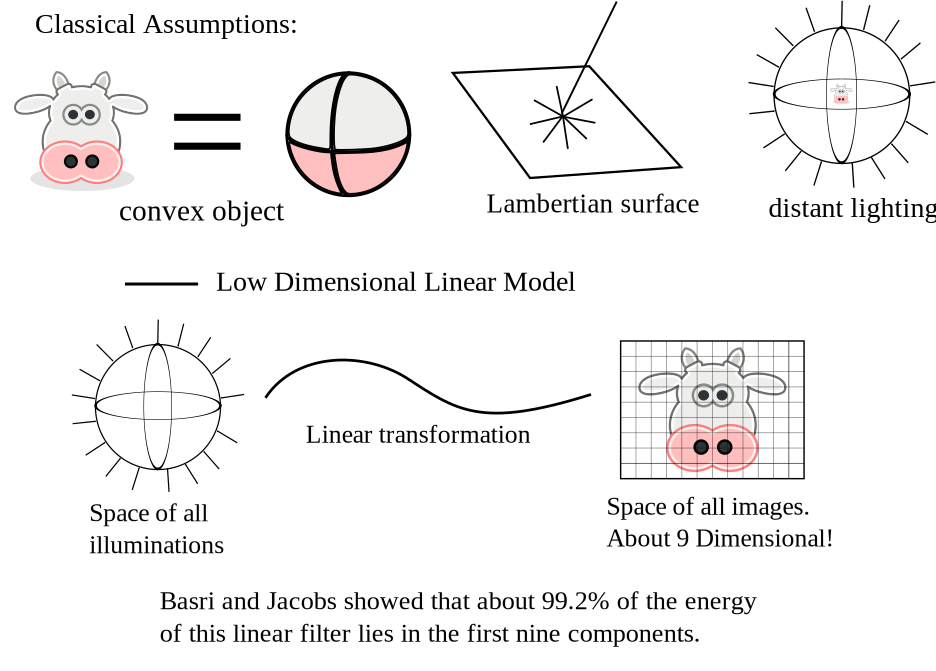
\includegraphics[height=0.8\textheight]{images/linear_illumination_model.pdf}
%}

\frame{
\frametitle{Linear Illumination Models}
\vspace{-5mm}\begin{center}
\includegraphics[width=0.3\textwidth]{images/shadow_example}
\end{center}\vspace{-5mm}
\begin{itemize}
\item Despite Shadowing and Specularities Images still linear WRT illumination
\item We can make Shadows and Specularities our Friends rather than our Enemies
\item {\em Experimentally} determine which training illuminations needed
\end{itemize}
}

\frame{
\frametitle{Acquisition System}

\includegraphics[width=0.3\textwidth]{images/camera_rig_drawings/perspective.pdf}

Projector-Based System:
\begin{itemize}
\item Easy to re-configure projector geometry
\item Trivial to change illumination patterns
\item Easier to construct and deploy
\item Very complete angular illumination coverage
\end{itemize}
}

\frame{
\frametitle{Training Illumination Rig}
\begin{columns}
\begin{column}{.5\textwidth}
\begin{center}
Side View\\
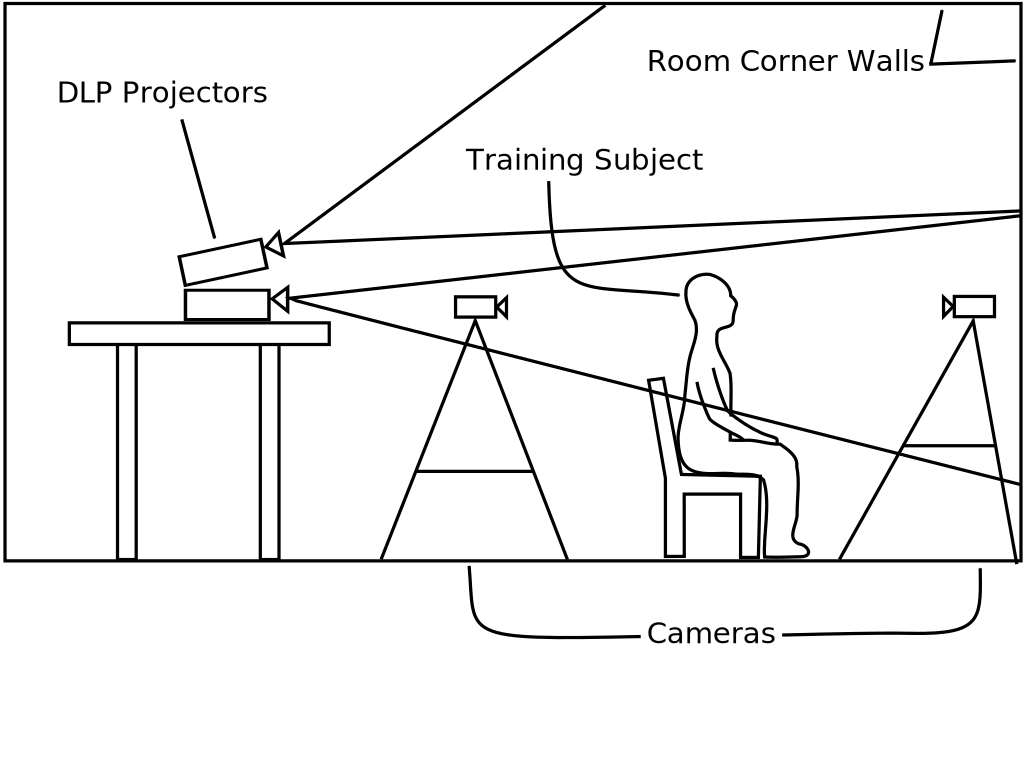
\includegraphics[width=\textwidth]{images/camera_rig_drawings/coverage_side.pdf}
\end{center}
\end{column}
\begin{column}{.5\textwidth}
\begin{center}
Top View\\
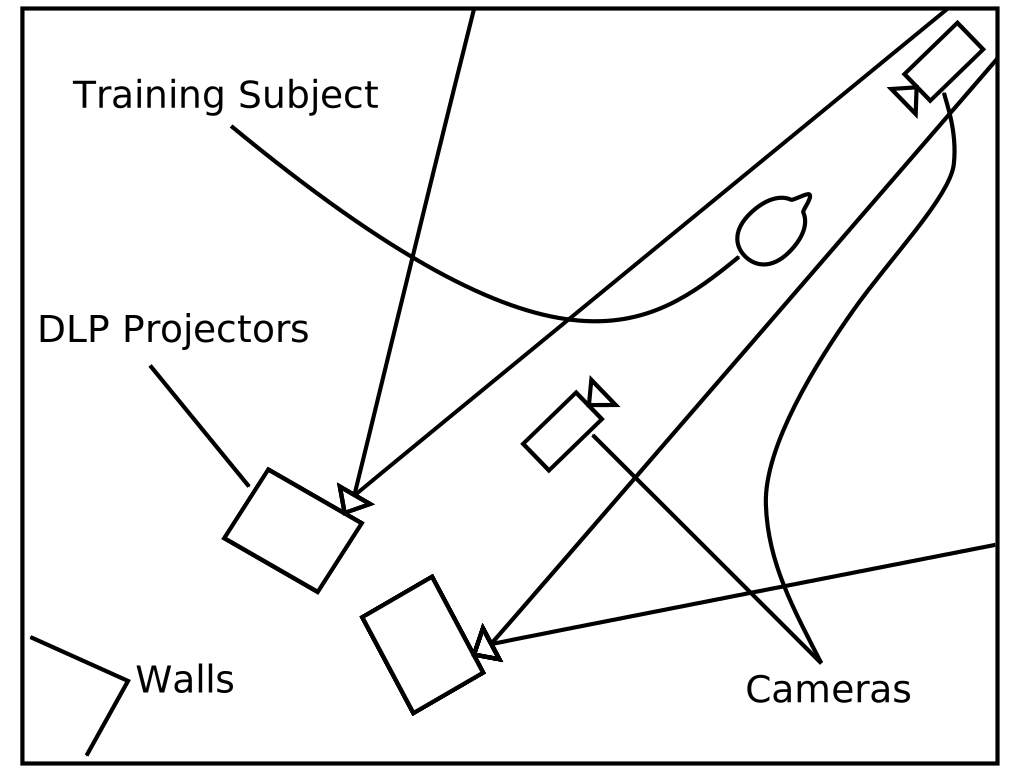
\includegraphics[width=\textwidth]{images/camera_rig_drawings/coverage_top.pdf}
\end{center}
\end{column}
\end{columns}
}

\frame{
\renewcommand{\imagesizestring}{height}
\setlength{\imagesizea}{0.41\textheight}
\frametitle{Experimentally Motivated Illumination Set}
\begin{tabular}{cc}

\includegraphics[\imagesizestring = \imagesizea]{images/camera_rig_drawings/side_front.pdf} & \includegraphics[\imagesizestring = \imagesizea]{images/illuminations/front.png}\\

\includegraphics[\imagesizestring = \imagesizea]{images/camera_rig_drawings/side_back.pdf} & \includegraphics[\imagesizestring = \imagesizea]{images/illuminations/back.png}
\end{tabular}
}

%\frame{\frametitle{Sample Training Images, Originals}
%\includegraphics[width=\textwidth]{images/training_contact_sheet.png}
%}

%\subsection{Alignment}
%\frame{\tableofcontents[currentsection, currentsubsection]}
%\frame{\frametitle{Compound Effect of Alignment and Illumination}
%\renewcommand{\imagesizestring}{height}
%\renewcommand{\imagesizea}{0.25\textheight}
%\renewcommand{\imagesizeb}{0.15\textheight}
%\renewcommand{\gapsizea}{-0mm}
\begin{tabular}[b]{cc@{}b{.5\textwidth}}
% Example for setting the heights of the images
\includegraphics[height=0.25\textheight]{figures_cvpr/promo/case1/detector.png}& \hspace{0.0mm}
\includegraphics[height=0.25\textheight]{figures_cvpr/promo/case1/sci_with_axis_face_case1.png} & 
{\bf Poor alignment}, Sufficient training illuminations \vfill\\
\includegraphics[height=0.25\textheight]{figures_cvpr/promo/alignment_and_detector.png}& \hspace{0.0mm}
\includegraphics[height=0.25\textheight]{figures_cvpr/promo/case2/sci_with_axis_face_case2.png} & 
{{\bf Good alignment}, Insufficient training illuminations}\vfill\\
\includegraphics[height=0.25\textheight]{figures_cvpr/promo/case3/alignment.png} & \hspace{0.0mm}
\includegraphics[height=0.25\textheight]{figures_cvpr/promo/case3/sci_with_axis_face_case3.png} &
{{\bf Good alignment}, Sufficient training illuminations}\vfill
\end{tabular}
}


\frame{
\frametitle{Image Embedding}
\vspace{-3mm}
\begin{center}
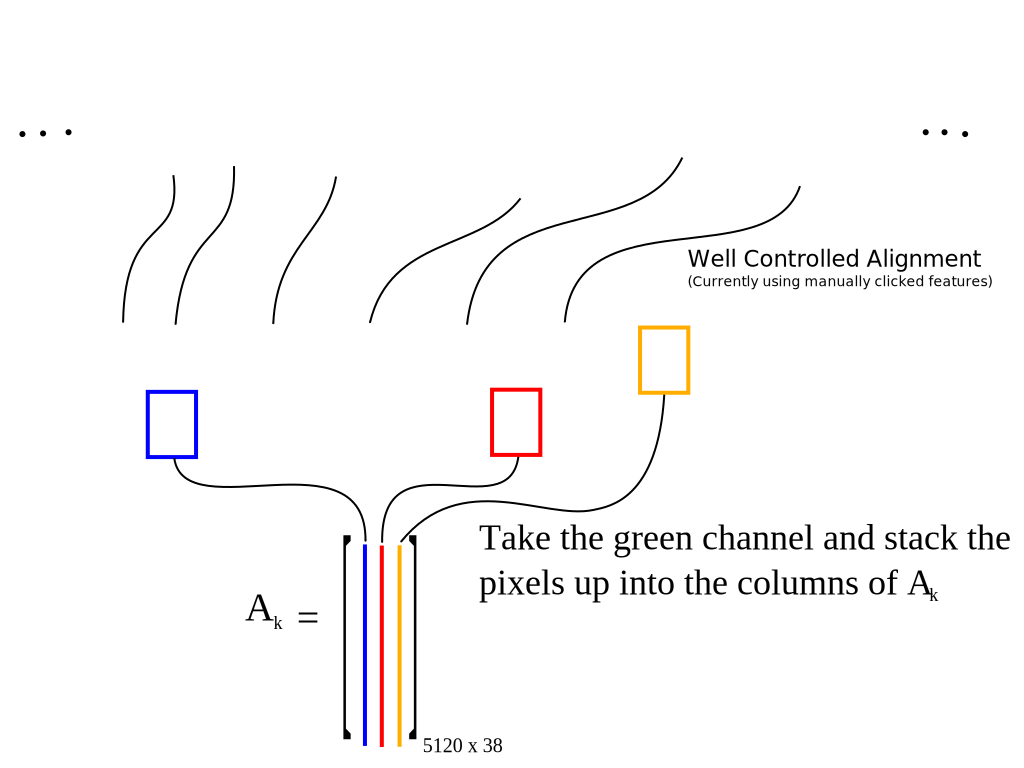
\includegraphics[width=.50\textwidth]{figures_embedding/training_embedding.pdf}\\
$A = [ A_1 \mid A_2 \mid \dots \mid A_K ] \in \Re^{m \times n}$
\end{center}
}


\frame{
\frametitle{Recognition Pipeline}
\begin{equation*}
(\hat \x, \hat \e,\hat \tau_i) = \argmin{\x,\e,\tau_i \in T} \| \e \|_1 \quad \subj \quad \y \circ \tau_i = A_i \x + \e
\end{equation*}
\begin{center}
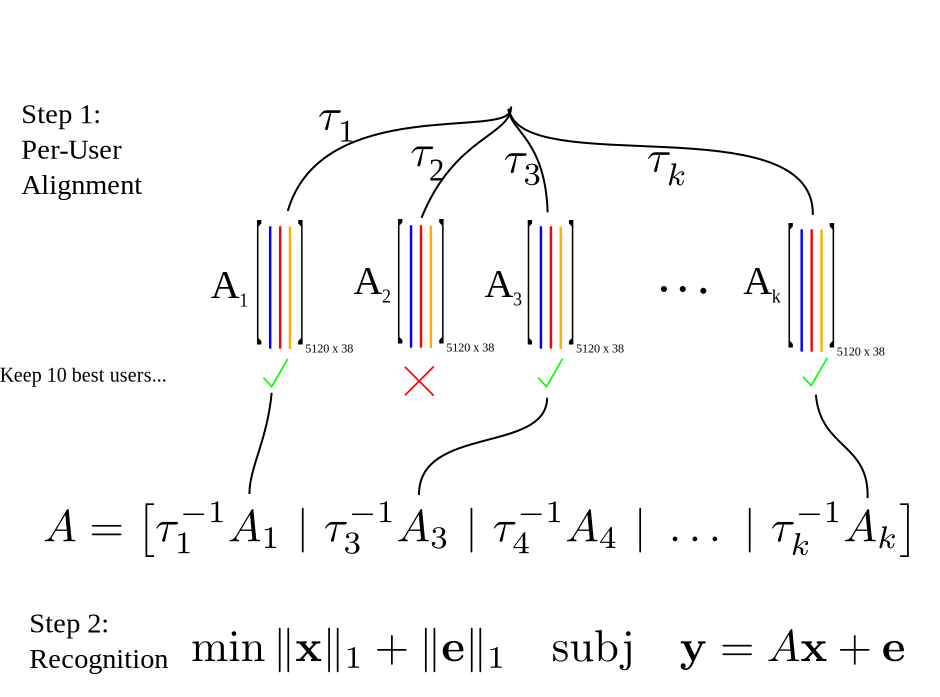
\includegraphics[width=.75\textwidth]{figures_embedding/pipeline.pdf}
\end{center}
}


%\frame{\frametitle{Alignment Examples}
%$\ell^1$ and $\ell^2$ minimization alignment comparison
%\begin{columns}
%\begin{column}{0.5\textwidth}
%\renewcommand{\imagesizestring}{height}
%\setlength{\imagesizea}{0.2\textheight}
%\begin{tabular}[t]{@{}c@{}c@{}c@{}c@{}m{.2\textwidth}}
%\includegraphics[\imagesizestring=\imagesizea]{figures_cvpr/L1_cropped} &
%\includegraphics[\imagesizestring=\imagesizea]{figures_cvpr/y_warp_L1} &
%\includegraphics[\imagesizestring=\imagesizea]{figures_cvpr/y_hat_L1} &
%\includegraphics[\imagesizestring=\imagesizea]{figures_cvpr/e_L1} &
%$\|\e\|_1$\\[-.05in]
%\includegraphics[\imagesizestring=\imagesizea]{figures_cvpr/L2_cropped} &
%\includegraphics[\imagesizestring=\imagesizea]{figures_cvpr/y_warp_L2} &
%\includegraphics[\imagesizestring=\imagesizea]{figures_cvpr/y_hat_L2} &
%\includegraphics[\imagesizestring=\imagesizea]{figures_cvpr/e_L2} &
%$\|\e\|_2$ \\[-.1in]
%{\tiny Face Boundary} & {\tiny Aligned Test} & {\tiny Reconstruction} & {\tiny $|$Error$|$}
%\end{tabular}
%\end{column}
%\begin{column}{0.5\textwidth}
%\renewcommand{\imagesizestring}{height}
%\setlength{\imagesizea}{0.2\textheight}
%Alignment tolerance for out-of-plane pose variation
%\includegraphics[\imagesizestring=\imagesizea]{figures_cvpr/21}
%\includegraphics[\imagesizestring=\imagesizea]{figures_cvpr/19}
%\includegraphics[\imagesizestring=\imagesizea]{figures_cvpr/17}
%\includegraphics[\imagesizestring=\imagesizea]{figures_cvpr/15}
%\includegraphics[\imagesizestring=\imagesizea]{figures_cvpr/13}\\
%\includegraphics[\imagesizestring=\imagesizea]{figures_cvpr/11}
%\includegraphics[\imagesizestring=\imagesizea]{figures_cvpr/09}
%\includegraphics[\imagesizestring=\imagesizea]{figures_cvpr/7}
%\includegraphics[\imagesizestring=\imagesizea]{figures_cvpr/5}
%\includegraphics[\imagesizestring=\imagesizea]{figures_cvpr/3}\\
%Alignment using a projective transformation works up to about $45^{\circ}$.
%\end{column}
%\end{columns}
%}


\renewcommand{\imagesizestring}{height}
\setlength{\imagesizea}{0.36\textheight}
\setlength{\gapsizea}{-0mm}
\frame{\frametitle{Alignment region of attraction}
%\begin{tabular}{cc}
\begin{center}
\includegraphics[\imagesizestring=\imagesizea]{figures_cvpr/promo/alignment_and_detector.png}
\includegraphics[\imagesizestring= \imagesizea]{figures_cvpr/translation_fig3.png}
\includegraphics[\imagesizestring= \imagesizea]{figures_cvpr/translation_rotation_fig1.png}
\end{center}
%\end{tabular}
\vspace{0mm}
{\tiny
\begin{itemize}
\item Translation is expressed as a fraction of outer eye corner distance.
\item In-plane rotation is expressed in degrees. 
\item Probability of convergence from synthetic transformations to hand-clicked ground truth
\item Training: CMU Multi-PIE, 120 subjects, 11 illuminations, session 2.  Re-sampled to $60 \times 80$ pixels.
\item Testing: 1 new illumination from session 3
\item Viola Jones' face detector average error on this data set falls safely within our region of attraction
\end{itemize}}
}


%\frame{\frametitle{Alignment Examples}
%{\footnotesize
%\vspace{-.1in}
%Comparison of $\ell^1$ and $\ell^2$ minimization:
%\renewcommand{\imagesizestring}{height}
%\setlength{\imagesizea}{0.15\textheight}
%\vspace{-.05in}
%\begin{center}
%\begin{tabular}[t]{b{.3in}cccc}
%$\min \|\e\|_2$\vfill &
%\includegraphics[\imagesizestring=\imagesizea]{figures_cvpr/L2_cropped} &
%\includegraphics[\imagesizestring=\imagesizea]{figures_cvpr/y_warp_L2} &
%\includegraphics[\imagesizestring=\imagesizea]{figures_cvpr/y_hat_L2} &
%\includegraphics[\imagesizestring=\imagesizea]{figures_cvpr/e_L2} \\
%$\min \|\e\|_1$\vfill &
%\includegraphics[\imagesizestring=\imagesizea]{figures_cvpr/L1_cropped} &
%\includegraphics[\imagesizestring=\imagesizea]{figures_cvpr/y_warp_L1} &
%\includegraphics[\imagesizestring=\imagesizea]{figures_cvpr/y_hat_L1} &
%\includegraphics[\imagesizestring=\imagesizea]{figures_cvpr/e_L1} \\
%& {\tiny Face Boundary} & {\tiny Aligned Test} & {\tiny Reconstruction} & {\tiny $|$Error$|$}
%\end{tabular}
%\end{center}

%$\ell^1$ and $\ell^2$ minimization alignment comparison
%\renewcommand{\imagesizestring}{height}
%\setlength{\imagesizea}{0.15\textheight}
%\vspace{-.1in}

%%Alignment tolerance for out-of-plane pose variation
%Alignment using a projective transformation works up to about $45^{\circ}$.
%\vspace{-.05in}
%\begin{center}
%\includegraphics[\imagesizestring=\imagesizea]{figures_cvpr/21}
%\includegraphics[\imagesizestring=\imagesizea]{figures_cvpr/19}
%\includegraphics[\imagesizestring=\imagesizea]{figures_cvpr/17}
%\includegraphics[\imagesizestring=\imagesizea]{figures_cvpr/15}
%\includegraphics[\imagesizestring=\imagesizea]{figures_cvpr/13}\\
%\includegraphics[\imagesizestring=\imagesizea]{figures_cvpr/11}
%\includegraphics[\imagesizestring=\imagesizea]{figures_cvpr/09}
%\includegraphics[\imagesizestring=\imagesizea]{figures_cvpr/7}
%\includegraphics[\imagesizestring=\imagesizea]{figures_cvpr/5}
%\includegraphics[\imagesizestring=\imagesizea]{figures_cvpr/3}\\
%\end{center}}
%}

\frame{\frametitle{Large Scale Multi PIE experiments}
\begin{center}
\begin{tabular}{|l|c|c|c|c|}
\hline
Rec. Rates & Session 2 & Session 3 & Session 4  \\
\hline
\hline
LDA$_d$ (LDA$_m$) & 5.1 (49.4)\%  & 5.9 (44.3)\% & 4.3 (47.9)\%  \\
\hline
NN$_d$ (NN$_m$)  & 26.4 (67.3)\% & 24.7 (66.2)\% & 21.9 (62.8)\%  \\
\hline
NS$_d$ (NS$_m$) &  30.8 (77.6)\% & 29.4 (74.3)\% & 24.6 (73.4)\% \\
\hline
{Algorithm 1} & {\bf 91.4} \% & {\bf 90.3} \% & {\bf 90.2} \% \\
\hline
\end{tabular}
\end{center}
\begin{columns}
\begin{column}{0.5\textwidth}
\begin{itemize}
{\footnotesize
\item Training: all 249 subj. from session 1\\7 frontal illuminations
\item Testing: all users, from sessions 2-4\\ all 20 illuminations 
\item Use the 88 users not in session 1 for validation
\item Our Algorithm 1 used face detector; no manual intervention
\item subscript m for manual alignment, subscript d for detector
\item neutral expression
}
\end{itemize}
\end{column}
\begin{column}{0.5\textwidth}
\begin{center}
\includegraphics[width=\textwidth]{figures_cvpr/roc3.png}
\end{center}
\end{column}
\end{columns}
}


%\renewcommand{\imagesizestring}{width}
%\setlength{\imagesizea}{0.16\textwidth}
%\frame{
%\frametitle{Representative examples of failed Multi-PIE subjects}
%\includegraphics[\imagesizestring =\imagesizea]{figures_cvpr/079_01_01_051_08.png} 
%\includegraphics[\imagesizestring =\imagesizea]{figures_cvpr/130_01_01_051_08.png}
%\includegraphics[\imagesizestring =\imagesizea]{figures_cvpr/163_01_01_051_08.png} 
%\includegraphics[\imagesizestring =\imagesizea]{figures_cvpr/175_01_01_051_08.png} 
%\includegraphics[\imagesizestring =\imagesizea]{figures_cvpr/118_01_01_051_08.png} 
%\includegraphics[\imagesizestring =\imagesizea]{figures_cvpr/223_01_01_051_08.png}\\
%\includegraphics[\imagesizestring =\imagesizea]{figures_cvpr/079_02_01_051_08.png} 
%\includegraphics[\imagesizestring =\imagesizea]{figures_cvpr/130_02_01_051_08.png} 
%\includegraphics[\imagesizestring =\imagesizea]{figures_cvpr/163_02_01_051_08.png} 
%\includegraphics[\imagesizestring =\imagesizea]{figures_cvpr/175_02_01_051_08.png} 
%\includegraphics[\imagesizestring =\imagesizea]{figures_cvpr/118_02_01_140_08.png} 
%\includegraphics[\imagesizestring =\imagesizea]{figures_cvpr/223_02_01_140_08.png}\\
%Trouble when large changes in the appearance between training and testing
%\begin{itemize}
%\item Hair color, hair style
%\item Eyeglasses
%\item Facial Hair
%\end{itemize}
%}

% Experiments on our own training images

\renewcommand{\imagesizestring}{width}
\setlength{\imagesizea}{0.2\textwidth}
\frame{\frametitle{Experiments on our data set}
\small{
Training (common to all): 74 users, 38 images per user
\includegraphics[\imagesizestring =\imagesizea]{figures_cvpr/examples/1/DSC_1319.JPG} 
\includegraphics[\imagesizestring =\imagesizea]{figures_cvpr/examples/1/DSC_1531.JPG} 
\includegraphics[\imagesizestring =\imagesizea]{figures_cvpr/examples/1/DSC_1574.JPG} 
\includegraphics[\imagesizestring =\imagesizea]{figures_cvpr/examples/1/DSC_1622.JPG} 
\includegraphics[\imagesizestring =\imagesizea]{figures_cvpr/examples/1/DSC_1786.JPG}\\
Testing: 242 images of 47 subjects, no glasses, frontal view $\Rightarrow \textbf{\color{red} 95.9\%}$ recognition.
\includegraphics[\imagesizestring =\imagesizea]{figures_cvpr/examples/2/DSC_1448.JPG} 
\includegraphics[\imagesizestring =\imagesizea]{figures_cvpr/examples/2/DSC_1585.JPG} 
\includegraphics[\imagesizestring =\imagesizea]{figures_cvpr/examples/2/DSC_1588.JPG} 
\includegraphics[\imagesizestring =\imagesizea]{figures_cvpr/examples/2/DSC_1666.JPG} 
\includegraphics[\imagesizestring =\imagesizea]{figures_cvpr/examples/2/DSC_1874.JPG}\\
Testing: 109 images of 23 subjects with eyeglasses  $\Rightarrow \textbf{\color{red} 91.5\%}$ recognition.
\includegraphics[\imagesizestring =\imagesizea]{figures_cvpr/examples/3/DSC_1572.JPG} 
\includegraphics[\imagesizestring =\imagesizea]{figures_cvpr/examples/3/DSC_1587.JPG} 
\includegraphics[\imagesizestring =\imagesizea]{figures_cvpr/examples/3/DSC_1623.JPG} 
\includegraphics[\imagesizestring =\imagesizea]{figures_cvpr/examples/3/DSC_1652.JPG} 
\includegraphics[\imagesizestring =\imagesizea]{figures_cvpr/examples/3/DSC_1675.JPG}\\
Testing: 19 images of 14 subjects with sunglasses $\Rightarrow \textbf{\color{red}63.2\%}$ recognition.
}}


%\subsection{Contiguous Occlusion}
%\frame{\tableofcontents[currentsection, currentsubsection]}

\renewcommand{\imagesizestring}{height}
\setlength{\imagesizea}{0.25\textheight}
\setlength{\imagesizeb}{0.15\textheight}

\frame{\frametitle{SRC on Random Corruption}
\renewcommand{\imagesizestring}{height}
\setlength{\imagesizea}{0.10\textheight}
\vspace{-.1in}
\begin{itemize}
\item<1-> SRC is provably optimal for {\em randomized} corruption. 
\begin{center}
\begin{columns}
\begin{column}{0.5\textwidth}
%{\footnotesize Yale Dataset, 19 images per person:}
\begin{center}
\begin{tabular}{@{}cccc@{}}
\includegraphics[\imagesizestring=\imagesizea]{IEEEPAMI_Occlusion/figures/ysp-30-125-o.pdf} &
\includegraphics[\imagesizestring=\imagesizea]{IEEEPAMI_Occlusion/figures/ysp-30-125-e.pdf} &
\includegraphics[\imagesizestring=\imagesizea]{IEEEPAMI_Occlusion/figures/ysp-30-125-w.pdf} &
\includegraphics[\imagesizestring=\imagesizea]{IEEEPAMI_Occlusion/figures/ysp-30-125-r.pdf} \\[-.05in]
\includegraphics[\imagesizestring=\imagesizea]{IEEEPAMI_Occlusion/figures/ysp-50-379-o.pdf} &
\includegraphics[\imagesizestring=\imagesizea]{IEEEPAMI_Occlusion/figures/ysp-50-379-e.pdf} &
\includegraphics[\imagesizestring=\imagesizea]{IEEEPAMI_Occlusion/figures/ysp-50-379-w.pdf} &
\includegraphics[\imagesizestring=\imagesizea]{IEEEPAMI_Occlusion/figures/ysp-50-379-r.pdf} \\[-.05in]
\includegraphics[\imagesizestring=\imagesizea]{IEEEPAMI_Occlusion/figures/ysp-70-80-o.pdf} &
\includegraphics[\imagesizestring=\imagesizea]{IEEEPAMI_Occlusion/figures/ysp-70-80-e.pdf} &
\includegraphics[\imagesizestring=\imagesizea]{IEEEPAMI_Occlusion/figures/ysp-70-80-w.pdf} &
\includegraphics[\imagesizestring=\imagesizea]{IEEEPAMI_Occlusion/figures/ysp-70-80-r.pdf}\\[-.1in]
{\tiny Test Image} & {\tiny Error} & {\tiny Coefficients} & {\tiny Reconstruction}
\end{tabular}
\end{center}
\end{column}
\begin{column}{0.5\textwidth}
\begin{center}
\includegraphics[height=.3\textheight]{IEEEPAMI_Occlusion/figures/yb_result_rc.pdf}\\
\end{center}
\end{column}
\end{columns}

\end{center}
%\vspace{.3in}
\item<2-> For contiguous occlusion, SRC can handle up to 30\% occlusion.\\
\begin{columns}
\begin{column}{0.5\textwidth}
\begin{center}
\begin{tabular}{@{}cccc@{}}
\includegraphics[\imagesizestring=\imagesizea]{IEEEPAMI_Occlusion/figures/352-30-O.PDF} &
\includegraphics[\imagesizestring=\imagesizea]{IEEEPAMI_Occlusion/figures/352-30-E.PDF}&
\includegraphics[\imagesizestring=\imagesizea]{IEEEPAMI_Occlusion/figures/352-30-W.PDF}&
\includegraphics[\imagesizestring=\imagesizea]{IEEEPAMI_Occlusion/figures/352-30-R.PDF} \\[-.05in]
\includegraphics[\imagesizestring=\imagesizea]{IEEEPAMI_Occlusion/figures/395-30-O.PDF} &
\includegraphics[\imagesizestring=\imagesizea]{IEEEPAMI_Occlusion/figures/395-30-E.PDF}&
\includegraphics[\imagesizestring=\imagesizea]{IEEEPAMI_Occlusion/figures/395-30-W.PDF} &
\includegraphics[\imagesizestring=\imagesizea]{IEEEPAMI_Occlusion/figures/395-30-R.PDF}\\[-.05in]
{\tiny Test Image} & {\tiny Error} & {\tiny Coefficients} & {\tiny Reconstruction}
\end{tabular}
\end{center}
\end{column}
\begin{column}{0.5\textwidth}
\begin{center}
\includegraphics[height=.3\textheight]{IEEEPAMI_Occlusion/figures/yb_result_bab.pdf}
\end{center}
\end{column}
\end{columns}
\item<2-> Can we do better for spatially contiguous occlusions?
\end{itemize}
}

\frame{\frametitle{Markov Random Field Model}
\vspace{-.1in}
\begin{center}
\includegraphics[width=.35\textwidth]{images/lattice.pdf}\\
\vspace{-.15in}{\tiny Markov Random Field (MRF)}
\end{center}
\vspace{-.1in}
\begin{itemize}
\item Represent the image domain as an adjacency graph $G=(V,E)$
\item Let $\s$ be the support of $\e[i]$
\item Use classical Ising Model as statistical model for $\s$:\\
Model probability of adjacent pixels agreeing, and probability of pixel being occluded.
\end{itemize}
}

\frame{\frametitle{Solving Sparse Representation under MRF assumption}
\begin{itemize}
\item Want to solve 
$\hat \s = \mbox{arg}\max_{\x_k,\e,\s} p(\s, \e) \quad \mbox{s.t.} \quad \y = A_k \x_k + \e.$
\item Difficult non-convex optimization problem!
\item $\Rightarrow$ alternate between: 
\begin{enumerate} 
\item Solving SRC on the image region currently defined by $\s$:
	\begin{equation*}(\hat{\x}_k,\hat{\e}^*) = \argmin{\x,\e^*} \|\e^*\|_1  \; \textup{ s.t. } \; \y^* = A_k^*\x+\e^*, \x\geq 0 \end{equation*}
\item Using graph cuts and our statistical model do update $\s$:
	\begin{equation*} \hat{\s} = \argmax{\s \in \{-1,1\}^m}  \sum_{(i,j)\in E}  \lambda \s[i]\s[j] + \sum_{i\in V} \log p(\e[i] | \s[i]).\end{equation*}
\end{enumerate}
\end{itemize}
}

%\frame{\frametitle{The Complete MRF Recognition Algorithm}
%{\footnotesize
%\begin{algorithmic}[1]
%\STATE {\bf Input:} A matrix of normalized training samples $A =
%[A_1,A_2,\ldots,A_K] \in \Re^{m\times n}$ for $K$ classes, a test
%sample $\y \in \Re^{m}$.

%\FOR{each subject $k$}

%\STATE Initialize the error support $\s^{(0)}_k = \mathbf{-1}_m$.

%\STATE {\bf repeat}

%\STATE \hspace{3mm}$A_k^* = A_k[\s^{(t-1)}_k=-1,\, :\, ]$, $\y^* =
%\y[s^{(t-1)}_k=-1]$;

%\STATE \hspace{3mm}Solve the convex program\\
%\hspace{5mm} $(\hat{\x}_k,\hat{\e}^*) \;=\; \arg\min \|\e^*\|_1 $\\
%\hspace{24mm} $\mathrm{ s.t. } \quad \y^* = A_k^*\x+\e^*, \, \x\geq 0;$

%\STATE \hspace{3mm}$\hat{\e}_k\leftarrow \y-A_k\hat{\x}_k$;

%\STATE \hspace{3mm}Update error support via graph cuts:\vspace{0mm}
%$$\s^{(t)}_k = \arg\hspace{-4mm}\max_{\s\in\{-1,1\}^m}\hspace{-2mm}\sum_{i,j\in
%E}\hspace{-2mm}{\lambda} \s[i]\s[j]+\sum_{i\in
%V}\log\big(p(\hat{\e}_k[i]|\s[i])\big);$$\vspace{0mm}
%\STATE {\bf until} maximum iterations or convergence.

%\STATE Compute the normalized error $$\mathbf{r}_k(\y) =
%\frac{\|\y^*-A_k^*\hat{\x}_k\|_1}{|\{ i \mid \s_k[i] = -1 \}|^2}. \vspace{0mm}$$
%\ENDFOR

%\STATE {\bf Output:} identity$(\y) = \arg\min_k \r_k(\y)$.
%\end{algorithmic}
%}}

%\frame{\frametitle{Choosing Model Parameters}
%\begin{itemize}
%\item Meaning of $\tau$ and $\lambda$: \begin{itemize}\item larger $\lambda$ smoothes $\s$ at the expense of increasing $\e$. \item $\tau$ is a threshold on $\e$, above which pixel is considered occluded \end{itemize}
%\item For a given $\lambda$, the support of $\e$ will drop off suddenly as $\tau$ is decreased:
%\begin{center}\includegraphics[width=0.5\textwidth]{figures_iccv/n_of_goodentry.pdf}\end{center}
%\item{Beyond red point many unoccluded pixels get mis-labelled as occluded.}
%\end{itemize}
%}

\renewcommand{\imagesizestring}{height}
\setlength{\imagesizea}{0.15\textheight}
\frame{\frametitle{Tuning MRF Model Parameters}
Example test image from AR database, occluded by scarf: \\
\begin{center}
\fbox{\includegraphics[height=0.225\textheight]{figures_iccv/test_epsilon.png}}\\
\end{center}
Error support for varying $\lambda, \tau$:
\begin{tabular}{cccccccb{.120\textwidth}}
$\lambda = 1$ &
\fbox{\includegraphics[height=\imagesizea]{figures_iccv/epsilon1/20.png}}&
\fbox{\includegraphics[height=\imagesizea]{figures_iccv/epsilon1/17.png}}&
\fbox{\includegraphics[height=\imagesizea]{figures_iccv/epsilon1/14.png}}&
\fbox{\includegraphics[height=\imagesizea]{figures_iccv/epsilon1/11.png}}&
\fbox{\includegraphics[height=\imagesizea]{figures_iccv/epsilon1/8.png}}&
\fbox{\includegraphics[height=\imagesizea]{figures_iccv/epsilon1/5.png}}&
\fbox{\includegraphics[height=\imagesizea]{figures_iccv/epsilon1/2.png}}\\
$\lambda = 3$&
\fbox{\includegraphics[height=\imagesizea]{figures_iccv/epsilon3/20.png}}&
\fbox{\includegraphics[height=\imagesizea]{figures_iccv/epsilon3/17.png}}&
\fbox{\includegraphics[height=\imagesizea]{figures_iccv/epsilon3/14.png}}&
\fbox{\includegraphics[height=\imagesizea]{figures_iccv/epsilon3/11.png}}&
\fbox{\includegraphics[height=\imagesizea]{figures_iccv/epsilon3/8.png}}&
\fbox{\includegraphics[height=\imagesizea]{figures_iccv/epsilon3/5.png}}&
\fbox{\includegraphics[height=\imagesizea]{figures_iccv/epsilon3/2.png}}\\
 &$\tau=0.2$ & 0.17 & 0.14 & 0.11 & 0.08 & 0.05 & 0.02
\end{tabular}
}

\frame{\frametitle{MRF vs. SRC on Our Dataset}
\newcommand{\imagewidth}{.55in}
\vspace{-.12in}
{\tiny Training: 116 subjects, 38 images each, aligned using algorithm in previous section initialized by hand.}\\
\vspace{-.2in}
\begin{center}
\begin{tabular}{cccccc}
& {\small Normal} & {\small Eyeglasses} & {\small Sunglasses} & {\small Hats} & {\small Disguises} \\ [-.05in]
{\tiny \# Testing Images} & {\tiny 354} & {\tiny 118} & {\tiny 126} & {\tiny 40} & {\tiny 217}\\
& \includegraphics[width=\imagewidth]{figures_iccv/real_data_examples/normal_1.jpg} & \includegraphics[width=\imagewidth]{figures_iccv/real_data_examples/glasses_1.jpg} & \includegraphics[width=\imagewidth]{figures_iccv/real_data_examples/sunglasses_1.jpg} & \includegraphics[width= \imagewidth]{figures_iccv/real_data_examples/hats_1.jpg} & \includegraphics[width=\imagewidth]{figures_iccv/real_data_examples/disguise_1.jpg} \\
& \includegraphics[width=\imagewidth]{figures_iccv/real_data_examples/normal_2.jpg} & \includegraphics[width=\imagewidth]{figures_iccv/real_data_examples/glasses_2.jpg} & \includegraphics[width=\imagewidth]{figures_iccv/real_data_examples/sunglasses_2.jpg} & \includegraphics[width=\imagewidth]{figures_iccv/real_data_examples/hats_2.jpg} & \includegraphics[width=\imagewidth]{figures_iccv/real_data_examples/disguise_2.jpg} \\
& \includegraphics[width=\imagewidth]{figures_iccv/real_data_examples/normal_3.jpg} & \includegraphics[width=\imagewidth]{figures_iccv/real_data_examples/glasses_3.jpg} & \includegraphics[width=\imagewidth]{figures_iccv/real_data_examples/sunglasses_3.jpg} & \includegraphics[width=\imagewidth]{figures_iccv/real_data_examples/hats_3.jpg} & \includegraphics[width=\imagewidth]{figures_iccv/real_data_examples/disguise_3.jpg} \\
{\small MRF Recognition} & 91.4\% & 90.9\% & {\bf 81.0\%} & {\bf 55.0\%} & {\bf 43.6\%}\\
{\small SRC Recognition} & {\bf 99.4}\% & {\bf 98.3}\% & 65.6\% & 40.0\% & 37.8\%
\end{tabular}
\end{center}
}

\frame{\frametitle{Recap}
The proposed SRC based alignment and recognition algorithm is already:
\begin{itemize}
\item very robust to illumination variation
\item robust to minor occlusions
\item robust to large in-plane pose variation
\end{itemize}
Unfortunately:
\begin{itemize}
\item Performance still poor for moderate to severe occlusions
\item Way to slow for commercial applications in current state 
\end{itemize}
}

\frame{\frametitle{Recognition Pipeline Demonstration}
\begin{itemize}
\item Test image taken today
\item Training images taken over 1 year ago
\item 38 illuminations per subject, ??? subjects in gallery.
\item Implemented in OpenCV
\item Running on XYZ machine
\end{itemize}
}

\section{Improved Pipeline}
\frame{\tableofcontents[currentsection, currentsubsection]}

\subsection{Improved Face Window}
\frame{ \frametitle{Improved Face Window} 
\centering
\begin{tabular}{@{}cc@{}}
\includegraphics[trim=1.9in .7in 1.9in .5in, clip, height=1.8in]{../figures_pami/example.png} &
\includegraphics[trim=1.9in .7in 1.9in .5in, clip, height=1.8in]{../figures_pami/example_new.png} \\
Default window. & Proposed window.
\end{tabular}
\small
{\small Recognition rates on the Multi-PIE database for
different pairings of alignment and recognition stages:}
\begin{tabular}{|c|c|c|c|c|c|c|c|c|c|c| }
\hline
\backslashbox{Rec.}{Align.}
& \multicolumn{3}{|c|}{Face Detector}
& \multicolumn{3}{|c|}{Manual}
& \multicolumn{3}{|c|}{Iterative Alignment}
\\
\hline
Session $\rightarrow$	& 2		&3			&4			& 2		&3			&4			& 2		&3			&4		\\
\hline
NS	& 30.8\%	& 29.4\%	& 24.6\%	& 77.6\%	& 74.3\%	& 73.4\%	& 84.5\%	& 82.3\%	& 81.4\% \\
\hline
NN	& 26.4\%	& 24.7\%	& 21.9\%	& 67.3\%	& 66.2\%	& 62.8\%	& 73.5\%	& 69.6\%	& 69.3\% \\
\hline
LDA	& 5.1\%		& 5.9\%		& 4.3\%		& 49.4\%	& 44.3\%	& 47.9\%	& 91.0\%	& 89.9\%	& 88.1\% \\
\hline
LBP	& 39.9\%	& 38.1\%	& 33.9\%	& 93.3\%	& 91.2\%	& 92.9\%	& {\bf 95.2\%}	& {\bf 94.7\%}	& {\bf 93.5\%} \\
\hline
SRC	& -- & -- & -- & -- & -- & -- & 93.9\%	& 93.8\%	& 92.3\% \\
\hline
\end{tabular}
}

\subsection{Improved Occlusion Handling}

\frame{ \frametitle{Difficulty with MRF Model} 
MRF showed improved occlusion handling for the aligned case.
Unfortunately, when MRF model and iterative alignment are combined,
alignment stability problems arise.  The core problem: the algorithm
is unable to differentiate between the error caused by occlusion and
the error caused by initial misalignment. 
}

\frame{ \frametitle{Overlapping Block Model} 
\includegraphics[width=4in]{../figures_pami/occ_block.png}
In order to better handle sunglasses, try overlapping Block Model: 
Perform recognition on a set of reduced size windows (Blocks) that are:
\begin{itemize}
\item small enough to sometimes miss occlusions
\item large enough to converge independently
\end{itemize}
...and vote to complete the classification.
}

\newcommand{\tempwidth}{0.1667\textwidth}
\frame{ \frametitle{Robustness to Sunglasses} 
\centering
\begin{tabular}{@{}c@{}c@{}c@{}c@{}c@{}c@{}}
\includegraphics[width=\tempwidth,clip=true]{../figures_pami/uiuc_example/sunglasses/DSC_1565.JPG} &
\includegraphics[width=\tempwidth,clip=true]{../figures_pami/uiuc_example/sunglasses/DSC_3656.JPG} &
\includegraphics[width=\tempwidth,clip=true]{../figures_pami/uiuc_example/sunglasses/DSC_3827.JPG} &
\includegraphics[width=\tempwidth,clip=true]{../figures_pami/uiuc_example/sunglasses/DSC_4090.JPG} &
\includegraphics[width=\tempwidth,clip=true]{../figures_pami/uiuc_example/sunglasses/DSC_4106.JPG} &
\includegraphics[width=\tempwidth,clip=true]{../figures_pami/uiuc_example/sunglasses/DSC_4126.JPG} \\
\includegraphics[width=\tempwidth,clip=true]{../figures_pami/uiuc_example/sunglasses_failed/DSC_1611.JPG} &
\includegraphics[width=\tempwidth,clip=true]{../figures_pami/uiuc_example/sunglasses_failed/DSC_3528.JPG} &
\includegraphics[width=\tempwidth,clip=true]{../figures_pami/uiuc_example/sunglasses_failed/DSC_3744.JPG} &
\includegraphics[width=\tempwidth,clip=true]{../figures_pami/uiuc_example/sunglasses_failed/DSC_3995.JPG} &
\includegraphics[width=\tempwidth,clip=true]{../figures_pami/uiuc_example/sunglasses_failed/DSC_4030.JPG} &
\includegraphics[width=\tempwidth,clip=true]{../figures_pami/uiuc_example/sunglasses_failed/DSC_4095.JPG} \\
\end{tabular}
Top row: examples where the overlapping blocks method succeeded. 
Bottom row: examples where the overlapping blocks method failed.
}


\subsection{Updated Experiments on Large Datasets}


\frame{\frametitle{Large Scale Experiments on Multi-PIE}
{\small Recognition rates on the Multi-PIE database for
different pairings of alignment and recognition stages.}
\centerline{
\begin{tabular}{|c|c|c|c|c|c|c|c|c|c|c| }
\hline
\backslashbox{Rec.}{Align.}
& \multicolumn{3}{|c|}{Face Detector}
& \multicolumn{3}{|c|}{Manual}
& \multicolumn{3}{|c|}{Iterative Alignment}
\\
\hline
Session $\rightarrow$	& 2		&3			&4			& 2		&3			&4			& 2		&3			&4		\\
\hline
NS	& 30.8\%	& 29.4\%	& 24.6\%	& 77.6\%	& 74.3\%	& 73.4\%	& 84.5\%	& 82.3\%	& 81.4\% \\
\hline
NN	& 26.4\%	& 24.7\%	& 21.9\%	& 67.3\%	& 66.2\%	& 62.8\%	& 73.5\%	& 69.6\%	& 69.3\% \\
\hline
LDA	& 5.1\%		& 5.9\%		& 4.3\%		& 49.4\%	& 44.3\%	& 47.9\%	& 91.0\%	& 89.9\%	& 88.1\% \\
\hline
LBP	& 39.9\%	& 38.1\%	& 33.9\%	& 93.3\%	& 91.2\%	& 92.9\%	& {\bf 95.2\%}	& {\bf 94.7\%}	& {\bf 93.5\%} \\
\hline
SRC	& -- & -- & -- & -- & -- & -- & 93.9\%	& 93.8\%	& 92.3\% \\
\hline
\end{tabular}
A combination of iterative alignment and LBP achieves highest recognition rate.
}}

\frame{ \frametitle{Comparisons with LBP} 
\centerline{
\begin{tabular}{@{}cc@{}}
\includegraphics[height=2.5in]{../figures_pami/pami_roc_revision2} &
\includegraphics[height=2.5in]{../figures_pami/pami_roc2} \\
(a) & (b) \\
\end{tabular}
}
\small {\bf ROC curves} for subject validation on Multi-PIE database,
(a) for all algorithms with iterative alignment, and
(b) for the classical algorithms with manual alignment (indicated by a subscript ``m'').
}

\frame{ \frametitle{Improved performance on private dataset}
\centering 
Recognition rates on a more realistic private database.
\begin{tabular}{|c|c|c|c|c|}
\hline
Test Category & C1 & C2 & C3 & C4  \\
\hline
\hline
Recognition Rate & 98.4\% & 95.8\% & 95.1\% & 40.9\% \\
\hline
\end{tabular}
}


\section{Fast ALM Based Algorithms for $\ell_1$-Minimization}
\frame{\tableofcontents[currentsection, currentsubsection]}

\frame{ \frametitle{$\ell_1$ Minimization Algorithms} 
\begin{itemize}
\item Interior point method converges in small number of steps,  but each
step is very expensive, involves solving linear system and re-ordering data in inner loop.
\item To overcome this, a state-of-the-art
$\ell_1$-minimization solution based on \emph{augmented Lagrangian methods}
(ALM) [BertsekasD2003,YangA2010-ICIP] has been developed.
\item Belongs to family of iterative shrinkage-thresholding methods, contains only
first-order operations in its inner loop.
\end{itemize}
}

\frame{\frametitle{ALM Derivation}
Recall that the following minimization problem is used in the recognition stage:
\begin{equation}
\min_{\x, \e} \| \x \|_1 + \|\e\|_1 \quad \subj \quad \bb = A \x + \e.
\end{equation}
The corresponding augmented Lagrangian function is:
\begin{equation}
L_\mu (\x,\e,\blambda) = \|\x\|_1 + \|\e\|_1 + \langle \blambda, \bb-A\x - \e \rangle
+ \frac{\mu}{2} \|\bb - A\x - \e\|_2^2,
\end{equation}
where $\blambda$ is the Lagrange multiplier and $\mu > 0$ is a
penalty parameter. 
}

\frame{\frametitle{ALM Derivation}
The ALM method seeks a saddlepoint of $L_\mu
(\x,\e,\blambda)$ by alternating between optimizing with respect
to the primal variables $\x, \e$ and updating the dual variable
$\blambda$, with the other fixed, as follows:
\begin{equation}
\left \{
\begin{array}{lll}
(\x_{k+1},\e_{k+1})  =  \arg\min_{(\x,\e)} \, L_{\mu} (\x,\e,\blambda_k),\\
\blambda_{k+1}  =  \blambda_k + \mu (\bb - A\x_{k+1} - \e_{k+1}). \\
\end{array}
\right .
\label{eqn:alm}
\end{equation}
Although updating $\blambda$ is trivial,
minimizing $L_{\mu} (\x,\e,\blambda_k)$ with respect to both
$\x$ and $\e$ could still be costly. 
}

\frame{\frametitle{ALM Derivation} 
To further reduce the complexity of the
problem, we adopt an approach used in alternates between minimizing 
$L_{\mu} (\x,\e,\blambda_k)$ over $\x$ (with $\e$ fixed) and over $\e$ (with $\x$
fixed). After solving these two subproblems, the Lagrange multiplier $\blambda$
is updated, yielding an iteration of the form:
\begin{equation}
\left\{
\begin{array}{lll}
\e_{k+1}  =  \argmin{\e} L_{\mu} (\x_k,\e,\blambda_k) 
\x_{k+1}  =  \argmin{\x} \, L_{\mu} (\x,\e_{k+1},\blambda_k),\\
\blambda_{k+1}  =  \blambda_k + \mu (\bb - A\x_{k+1} - \e_{k+1}).
\end{array}
\right\}
\end{equation}
As the objective function is convex and alternation is between two
terms, this procedure is guaranteed to converge to a global optimum (see [YangJ2009-pp] and references therein).
}

\frame{\frametitle{ALM Derivation} 
In order to discuss the solution to the above subproblems, we
need to define the following soft-thresholding operator for a
vector $\x$ and a scalar $\alpha \geq 0$:
\begin{equation}
\mathcal{T}(\x,\alpha) = \textup{sign}(\x)\cdot \max \{|\x| - \alpha, 0\},
\end{equation}
where all the operations are performed component-wise. It is
easy to show that the subproblem with respect to $\e$ has a
closed-form solution given by the soft-thresholding operator:
\begin{equation}
\e_{k+1} = \mathcal{T}(\bb - A\x_k + \mu^{-1}\blambda_k, \mu^{-1}).
\end{equation}
}
 
\frame{\frametitle{ALM Derivation} 
To solve the subproblem associated with $\x$, we
apply a first-order $\ell^1$-minimization method,
called \emph{fast iterative shrinkage-threshold algorithm}
(FISTA) \cite{BeckA2009}. The main idea of FISTA is to
iteratively minimize a quadratic approximation $Q(\x, \z)$ to
$L_{\mu} (\x,\e_{k+1},\blambda_k)$ around a point $\z$, which is
carefully chosen in order to achieve a good convergence
rate. We summarize the entire ALM
algorithm as Algorithm~\ref{alg:alm}, where $\gamma$ denotes the
largest eigenvalue of the matrix $A^TA$. For the choice of parameter $\mu$, we take the same strategy as
in \cite{YangJ2009-pp} and set $\mu = 2m / \|\bb\|_1$.
}

\frame{
\frametitle{ALM for Global Recognition}
\begin{algorithmic}[1]
\begin{small}
\STATE {\bf Input:} $\bb \in \Re^m$, $A \in \Re^{m \times n}$,
$\x_1 = \mathbf{0}$, $\e_1 = \bb$, $\blambda_1 =
\mathbf{0}$.
\WHILE{not converged ($k = 1,2,\ldots$)}
\STATE $\e_{k+1} = \mathcal{T}\left(\bb - A\x_k +
\frac{1}{\mu}\blambda_k, \frac{1}{\mu}\right)$;
\STATE $t_1\leftarrow 1$, $\z_1 \leftarrow \x_k$, $\w_1 \leftarrow \x_k$;
\WHILE{not converged ($l = 1,2,\ldots$)}
\STATE $\w_{l+1} \leftarrow \mathcal{T}\left(\z_l +
\frac{1}{\gamma}A^T\left(\bb - A\z_l - \e_{k+1} +
\frac{1}{\mu}\blambda_k\right), \frac{1}{\mu\gamma}\right)$;
\STATE $t_{l+1} \leftarrow \frac{1}{2}\left( 1 +
\sqrt{1+4t_l^2}\right)$;
\STATE $\z_{l+1} \leftarrow \w_{l+1} + \frac{t_l - 1}{t_{l+1}}(\w_{l+1} - \w_l)$;
\ENDWHILE
\STATE $\x_{k+1} \leftarrow \w_{l}$,  \; $\blambda_{k+1} \leftarrow \blambda_k + \mu (\bb - A\x_{k+1} - \e_{k+1})$;
\ENDWHILE \STATE
{\bf Output:} $\x^* \leftarrow \x_k, \e^* \leftarrow \e_k$.
\end{small}
\end{algorithmic}
}

\frame{
\frametitle{ALM for Linearized Per-User Alignment}
The alignment stage requires the solution of the optimization problem:
\begin{equation}
\min_{\x, \e} \|\e\|_1 \quad \subj \quad \bb =
A \x + \e.
\end{equation}
The ALM derivation for this problem is very similar.
The augmented Lagrangian function is:
\begin{equation}
L_\mu (\x,\e,\blambda) = \|\e\|_1 + \langle \blambda, \bb-A\x - \e \rangle + \frac{\mu}{2} \|\bb - A\x - \e\|_2^2,
\end{equation}
For the alternating minimizations, the subproblem associated with $\e$
has the same closed-form solution as before, but the subproblem associated with
$\x$ can now be solved in closed form:
\begin{eqnarray}
\x^* &=& \argmin{\x} \langle \blambda, \bb-A\x - \e \rangle + \frac{\mu}{2} \|\bb - A\x - \e\|_2^2 \\
%\x^* = \argmin{\x} -\blambda^T A x + \frac{\mu}{2} (\x^T(A^T A) \x + 2(\e-\bb)^T A \x + (\e-\bb)^T (\e-\bb)) \\
%\x^* = \argmin{\x} -\blambda^T A x + \frac{\mu}{2} (\x^T(A^T A) \x + 2(\e-\bb)^T A \x) \\
%\x^* = \argmin{\x} (-\blambda^T -\bb -\frac{\blambda}{\mu}^T A x + \frac{1}{2} \x^T (A^T A) \x \\
0 &=& A^T(\e - \bb -\frac{\blambda}{\mu}) + (A^T A) \x^*\\
%(A^T A) \x^* =  A^T (\bb - \e + \frac{\blambda}{mu})\\
%\x^* =  (A^T A)^{-1} A^T (\bb - \e + \frac{\blambda}{mu})\\
\x^* &=&  A^\dagger (\bb - \e + \frac{\blambda}{\mu})
\end{eqnarray}
}

\frame{
\frametitle{ALM for Linearized Per-User Alignment}
\small
{\bf Input:} $\bb$, $A_i$, $\x_0 = \mathbf{0}$, $\tau_0$, and $J_0$.
\begin{algorithmic}[1]
\WHILE{not converged ($j = 1,2,\ldots$)}
\STATE Update $\bb_j \leftarrow \frac{\bb\circ \tau_{j-1}}{\|\bb\circ \tau_{j-1}\|}$; $B_j= [A_i, -J_{j-1}]$ and corresponding $(B_j^\dagger)^T$
\STATE Initialize $\ww_0 = \mathbf 0$, $\blambda_0 = \mathbf 0$
\WHILE{not converged ($k = 1,2,\ldots$)}
\STATE $\uu_0\leftarrow \ww_{k-1}$; $\zz_0\leftarrow \e_{k-1}$
\WHILE{not converged ($l = 1,2,\ldots$)}
\STATE $\zz_l \leftarrow \shrink\left(\bb_j - B_j\uu_{l-1} + \frac{\blambda_{k}}{\mu_{k-1}}, \frac{1}{\mu_{k-1}}\right)$
\STATE $\uu_l \leftarrow B_j^\dagger \left(\bb_j - \zz_{l} + \frac{\blambda_{k-1}}{\mu_{k-1}} \right) $
\ENDWHILE
\STATE $\ww_k \leftarrow \uu_l$; $\e_k \leftarrow \zz_l$
\STATE $\blambda_{k} \leftarrow \blambda_{k-1} + \mu_{k-1} (\bb_j - B_j\ww_{k} - \e_{k})$
\STATE $\mu_{k} \leftarrow \rho\mu_{k-1}$
\ENDWHILE
\STATE Update $\e_j$, $\tau_j$, and $J_j$
\ENDWHILE
\end{algorithmic}
{\bf Output:} $\tau_i^*\leftarrow \tau_j, \e_i^*\leftarrow \e_j$
}

%% INCORRECT???
%\frame{
%\frametitle{ALM for Iterative Alignment}
%\begin{algorithmic}[1]
%\begin{small}
%\STATE {\bf Input:} $\bb \in \Re^m$, $A \in \Re^{m \times n}$,
%$\x_1 = \mathbf{0}$, $\e_1 = \bb$, $\blambda_1 =
%\mathbf{0}$.
%\WHILE{not converged ($k = 1,2,\ldots$)}
%\STATE $\e_{k+1} = \mathcal{T}\left(\bb - A\x_k +
%\frac{1}{\mu}\blambda_k, \frac{1}{\mu}\right)$;
%\STATE $t_1\leftarrow 1$, $\z_1 \leftarrow \x_k$, $\w_1 \leftarrow \x_k$;
%\WHILE{not converged ($l = 1,2,\ldots$)}
%\STATE $\w_{l+1} \leftarrow \mathcal{T}\left(\z_l +
%\frac{1}{\gamma}A^T\left(\bb - A\z_l - \e_{k+1} +
%\frac{1}{\mu}\blambda_k\right), \frac{1}{\mu\gamma}\right)$;
%\STATE $t_{l+1} \leftarrow \frac{1}{2}\left( 1 +
%\sqrt{1+4t_l^2}\right)$;
%\STATE $\z_{l+1} \leftarrow \w_{l+1} + \frac{t_l - 1}{t_{l+1}}(\w_{l+1} - \w_l)$;
%\ENDWHILE
%\STATE $\x_{k+1} \leftarrow \w_{l}$,  \; $\blambda_{k+1} \leftarrow \blambda_k + \mu (\bb - A\x_{k+1} - \e_{k+1})$;
%\ENDWHILE \STATE
%{\bf Output:} $\x^* \leftarrow \x_k, \e^* \leftarrow \e_k$.
%\end{small}
%\end{algorithmic}
%}

%\frame{\frametitle{Complete ALM Algorithm}
%\begin{algorithmic}
%\WHILE{not converged}
%\WHILE{not converged}
%\STATE $[\e_{j+1}]_i  =  \shrink \left(\left[ \bb + \frac{1}{\mu_k}\blambda_k - A\x_j \right] _i, \frac{W_{ii}}{\mu_k}\right), \quad i = 1,2,\ldots,m$
%\STATE $t_1 \leftarrow 1$, $\z_1 \leftarrow \x_j$
%\WHILE{not converged}
%\STATE $\x_{l+1}  =  \shrink\left(\z_l - \frac{1}{\tau}A^T\left(A\z_l + \e_{j+1} - \bb - \frac{1}{\mu_k}\blambda_k\right), \frac{1}{\mu_k\tau}\right)$
%\STATE $t_{l+1} = 0.5\left( 1 + \sqrt{1+4t_l^2}\right)$
%\STATE $\z_{l+1} = \x_{l+1} + \frac{t_l - 1}{t_{l+1}}(\x_{l+1} - \x_l)$
%\ENDWHILE
%\ENDWHILE
%\STATE $\blambda_{k+1} = \blambda_k + \mu_k (\bb - A\x_{k+1} - \e_{k+1})$
%\STATE $\mu_{k+1} = \rho\cdot\mu_k$
%\ENDWHILE
%\end{algorithmic}
%}


\section{Parallel Implementations on CPU and GPU}
\frame{\tableofcontents[currentsection]}

\frame{ \frametitle{Introduction}
\begin{itemize}
\item ALM speeds up $\ell_1$ minimization...
\item ...but still need more speed!
\item This section presents parallelized implementations of the face pipeline
\item There is ample parallelism available in the pipeline
\item Leverage the high levels of concurrency available in multi-core CPU and GPU architectures.
\end{itemize}
}

\frame{ \frametitle{CPU vs. GPU Architecture Comparison}
\begin{itemize}
\item CPU: Intel E5530, Dual-socket, quad-core Xeon
\item GPU: Nvidia GTX480 Single-socket GPU on PCIe card
\end{itemize}

\centering
\begin{tabular}{l|c|c}
Attribute & CPU & GPU \\
\hline
Cache Size & {\color{red} 8MB} & 768 KB \\
Clock & {\color{red} 2.4 GHz} & 1.4 GHz \\
DRAM Bandwidth & 25 GB/s & {\color{red} 177 GB/s} \\
Vector Width & 4 & {\color{red} 64} \\
Cores	& 8 & {\color{red} 15} 
\end{tabular} 

\begin{itemize}
\item CPU has two levels of concurrency: {\em core-level} and {\em SSE-level}
\item GPU has two levels of concurrency: {\em SM-level} and {\em thread-level} 
\end{itemize}
}

\newcommand{\tempscale}[0]{0.8}
\frame{ \frametitle{CPU and GPU cache comparison}
\centering
The larger algorithm data structures: \\
\includegraphics[scale=\tempscale]{../figures_ijcb/arrays.pdf} \\
The caches on a E5530 CPU: \\
\includegraphics[scale=\tempscale]{../figures_ijcb/cpu_caches.pdf} \\
The caches on a GTX480 GPU: \\
\includegraphics[scale=\tempscale]{../figures_ijcb/gpu_caches.pdf} \\
}

%\frame{ \frametitle{Limitations of CUDA programming model}
%}

\frame{ \frametitle{Parallelization of SRC Recognition Stage}
\begin{itemize}
\item Single large $\ell_1$ minimization problem
\item Only one level of parallelism available: {\em pixel-level}
\item Essentially one essential parallelization strategy:\\
Map pixel-level parallelism onto both core-level and vector-level concurrency
\item Leverage built-in parallelization of MKL BLAS  and CUBLAS libraries
\item Array storage implicitly affects parallelization within the BLAS implementation
\end{itemize}
}
%\frame{ \frametitle{Parallelization of SRC Recognition Stage}
%\begin{itemize}
%\item Most operations map directly onto calls in the BLAS API.
%\item On the CPU, Intel's MKL BLAS can exploit both levels of concurrency on the CPU.
%\item On the GPU, Nvidia's CUBLAS exploits both levels of concurrency on the CPU.
%\item On the CPU, the remaining operations can be parallelized via manual threading (via OpenMP),
%and automatic vectorization (via the Intel ICC compiler).
%\item On the GPU, the remaining operations can be parallelized manually as CUDA kernels.
%\end{itemize}
%}


\frame{ \frametitle{Effect of Cache Size for solving a single minimization problem}
How does the speed of solving a single ALM problem at a time vary with problem size?
Benchmark the generic basis pursuit problem (alternate SRC formulation):
\begin{equation} 
\min \|\xx\|_1\quad \mbox{ subj. to }\quad \bb = A\xx
\end{equation}
{ \tiny
{\bf INPUT:} $\bb \in \Re^m$, $A=[A_1,\cdots, A_K] \in \Re^{m \times n}$, $\tau\leftarrow \max\mbox{eig}(A^TA)$, and constant $\rho>1$.
\begin{algorithmic}[1]
\WHILE{not converged ($k = 1,2,\ldots$)} 
\STATE $t_1 \leftarrow 1$, $\zz_1 \leftarrow \xx_k$, $\uu_1 \leftarrow \xx_k$ 
\WHILE{not converged ($l = 1,2,\ldots$)} 
\STATE $\uu_{l+1}  \leftarrow \shrink(\zz_l - \frac{1}{\tau}A^T(A\zz_l - \bb - \frac{1}{\mu_k}\blambda_k), \frac{1}{\mu_k\tau})$
\STATE $t_{l+1} \leftarrow \frac{1}{2}( 1 + \sqrt{1+4t_l^2})$
\STATE $\zz_{l+1} \leftarrow \uu_{l+1}+ \frac{t_l - 1}{t_{l+1}}(\uu_{l+1} - \uu_l)$ 
\ENDWHILE 
\STATE $\xx_{k+1} \leftarrow \uu_{l+1}$ 
\STATE $\blambda_{k+1} \leftarrow \blambda_k + \mu_k (\bb - A\xx_{k+1})$ 
\STATE $\mu_{k+1} \leftarrow \rho\cdot\mu_k$ 
\ENDWHILE 
\end{algorithmic}
{\bf OUTPUT:} $\xx^* \leftarrow \xx_k$.
}
}

\frame{ \frametitle{Effect of Cache Size for solving a single minimization problem}
{
\tiny
\begin{itemize}
\item Random Gaussian $A \in \Re^{m \times 2*m}$, with normalized columns
\item Ground truth $\x_0$ also random Gaussian, 10\% sparsity, normalized to unit norm
\item Measurement vector $\bb = A \x_0$.   
\item Termination when $\|\bx-\bx_0\| < \tau$ with $\tau=10^{-3}$.  
\item Running with single socket (4 cores, 8MB L3 cache).
\end{itemize}
}
\begin{center}
\includegraphics[width=3.5in]{../figures_ijcb/time_vs_matrix_size_constant_tol.pdf}
\end{center} 
Crossover point occurs exactly where A reaches 8MB L3 cache size!
}

\frame{ \frametitle{ALM Recognition Stage Benchmark}
Recognition stage runtime vs. face window resolution
Benchmark ALM based Recognition stage running on real data:
Images of 10 users from Iterative Alignment Stage, running on Multi-PIE.
Vary image size: $32\times32$, $48 \times 48$, $64 \times 64$, $96 \times
96$, and $128 \times 128$.  
\centering
{
	\includegraphics[width=3in]{../figures_ijcb/speedVsResolution.pdf} 
}
\begin{itemize}
\item Problem size too small to run efficiently on GPU.
\item Runtime for both implementations low compared to alignment stage.
\end{itemize}
}

\frame{ \frametitle{Parallelization of Iterative Alignment}
\begin{itemize}
\item Need to repeatedly solve many small $\ell_1$ minimization problems 
\item $\ell_1$ minimization is interleaved with image rewarping
\item Two levels of parallelism: \emph{problem-level} and \emph{pixel-level}
\end{itemize}
We consider two parallelizations of iterative alignment:
\begin{enumerate}
\item Alignment problems solved sequentially \\
\begin{itemize} 
\item problem-level parallelism unused
\item pixel-level parallelism mapped onto both vector-level and core-level hardware concurrency
\end{itemize}
\item Alignment problems solved concurrently \\
\begin{itemize} 
\item problem-level parallelism mapped onto core-level concurrency
\item pixel-level parallelism mapped onto vector-level concurrency
\end{itemize}
\end{enumerate}
}

\frame{ \frametitle{Parallelization of Iterative Alignment}
First, in order to measure the impact of solving many
$\ell_1$ problems-per concurrently on the GPU, we benchmark three implementations of the
alignment $\ell_1$-minimization solver with $A$ of size $5120 \times 32$, and a fixed
$50$ inner loop iterations for each of $50$ outer loop iterations. The runtime
on a GTX480 GPU is averaged over a large number of trials, which are run
sequentially or concurrently depending on the implementation.
The results are shown in Table \ref{tbl:ubench}.
Our proposed parallelization of the $\ell_1$-minimization used in the alignment
stage is {\em eight times} faster than an implementation solving a single
problem at a time using the stock BLAS libraries.
%\footnote{The streams implementation is limited significantly by a 
%cap on the number of concurrent streams in the current version of CUDA}
\centerline{
\small
\begin{tabular}{|l|c|}
\hline
Sequential solver using CUBLAS & 302\,ms \\
\hline
One problem per SM using CUDA streams & 70\,ms  \\
\hline
Four problems per SM using single kernel & {\bf 36\,ms} \\
\hline
\end{tabular} 
}
}

\frame{ \frametitle{Parallelized Alignment Stage Benchmark}
{
	\tiny
	\begin{itemize}
	\item CMU Multi-PIE Face Database with 249 users
	\item Gallery: Frontal images from session 1, 20 images per subject
	\item Test set: Frontal images from session 2 
	\item Alignment is performed using a $64 \times 64$ window
	\item similarity transformations with manual initialization 
	\end{itemize}
}
\centering
\includegraphics[width=3in]{../figures_ijcb/alignment_runtime_graph.pdf}
\begin{itemize}
\item Number of gallery subjects is varied to show scalability
\item {\em Much} faster than earlier results!
\item Recognition against 249 users in under 10s!
\end{itemize}
}

\frame{ \frametitle{Parallelized Pipeline Accuracy}
\centering
\includegraphics[width=4in]{../figures_ijcb/accuracyVsResolution.pdf} 
\begin{itemize}
\item Varied resolution of image resolution for recognition stage.
\item At the optimal resolution, the GPU implementation reaches 95\% recognition rate, the max
achievable given the selected recognition users.  
\item For significantly lower resolutions, the accuracy drops off significantly.  
\item The slight difference in CPU vs. GPU accuracy may be a result of numerical precision differences in matrix
inversion and vector reduction.
\end{itemize}
}

\frame{ \frametitle{Conclusion}
\begin{itemize}
\item On both CPU and GPU architectures, parallelizations of
ALM that solve multiple face alignment problems concurrently are significantly
faster than implementations than naive BLAS based implementations.
\item Thanks to more efficient use of faster hardware, dramatic speed improvements
over previous parallel implementation.
\item Achieved near real-time recognition performance on 8 core workstation, and 12+ core workstations are already available.
\item SM-level CUDA BLAS routines were painful to develop, but provide a foundation
for new $\ell_1$ solvers already under development.
\end{itemize}
Promising Future
\begin{itemize}
\item CPUs are increasing number of cores and vector widths
\item GPU are increasing in amount of cache
\item $\Rightarrow$ Both architectures converging towards an architectural balance
that is more conducive to face recognition.
\item AMD APU and Intel Knight's corner architectures are attempting to blend the best
aspects of CPU and GPU.
\end{itemize}
}



%\section{Conclusion and Future Work}
%%%\subsection{Recap}
%\frame{ \frametitle{Recap} By prelim had proposed a complete face recognition pipeline for face recognition,
%but it wasn't fast enough yet for commercial application}
%\frame{ \frametitle{Recap} Since prelim, have dramatically improved the speed of the system without sacrificing
%performance.}
%%%\subsection{Future Work}
%\frame{ \frametitle{Improve acquisition system using multiplexed illuminations } }
%\frame{ \frametitle{Merge iterative alignment, SRC, and LBP} }
%\frame{ \frametitle{Increase arithmetic intensity} Mention work in progress on subgradient descent methods.
%take advantage of tallness of the arrays, geometry of the $\ell_1$ minimization problem}

%\section[Conclusion]{Conclusion and Future Work}

\frame{ \frametitle{Conclusion} 
\begin{itemize}
\item Projector-based image acquisition system dramatically simplifies capture of subjects under many illuminations
\item Iterative alignment techniques achieve excellent robustness to alignment variations
\item Proposed promising techniques for improving robustness to severe occlusions 
\item Developed ALM based solvers that dramatically improve scalability of global representation
\item Designed and implemented highly optimized parallel solvers on CPU and GPU architectures
\end{itemize}
}

\frame{ \frametitle{Future Work: Improving pipeline speed} 
\begin{itemize}
\item Improve Recognition Speed
\begin{itemize}
\item On GPU, parallelized ALM implementations are bandwidth limited
\item Want to reduce number of loads of $A$ per iteration, \# of iterations
\item Can afford to spend more FLOPS on any subproblem that fits in cache
\end{itemize}
\item Try to leverage geometry of $\ell_1$ minimization problem:
\begin{itemize}
\item Exact line search only costs $m \log m$ with small constant
\item Expensive part of descent direction computation operates on $n \times n$ subarray
\item Multi-Scale within solver to leverage correlation of adjacent pixels
\end{itemize}
\item Faster training image acquisition 
\begin{itemize}
\item Multiplexed Illuminations can be used to increase SNR or decrease exposure time...
\item ...but require calibrated projectors.
\item Automatically calibrate projectors? 
\end{itemize}
\end{itemize}
}

\frame{ \frametitle{Future Work: Improving recognition performance} 
How can we perform iterative alignment even with severe occlusions?
\begin{itemize}
\item Explore alternative convex norms that encourage contiguous error (i.e. C-norm).
\item Attempt to distinguish between occlusion and misalignment error components.
\item Random initialization techniques [Yang, Shia] are investigating this in face tracking context.
\end{itemize}
Why does global representation (i.e. via SRC) improve imposter rejection so much?
\begin{itemize}
\item LBP achieves better R.R. but SRC has better ROC curve. 
\item CVPR paper from another group (under review) claims explanation for $\ell_2$ case, but result is flawed.
\end{itemize}
}


%\frame{
\frametitle{Publications}
{\bf Relevant Conference Papers}
{\scriptsize
\begin{itemize}
\item {\em Towards a Practical Face Recognition System: Robust
Registration and Illumination by Sparse Representation} ({\bf Andrew
Wagner}, John Wright, Arvind Ganesh, Zihan Zhou, Yi Ma) to appear in
CVPR, 2009
\item {\em Face Recognition with Contiguous Occlusion Using Markov
Random Fields} (Zihan Zhou, {\bf Andrew Wagner}, John Wright, Hossein
Mobahi, Yi Ma) submitted to ICCV, 2009
\end{itemize}}
{\bf Other Publications}
{\scriptsize
\begin{itemize}
\item {\em The Algebra and Statistics of Generalized Principal
Component Analysis} (Shankar Rao, Harm Derksen, Robert Fossum, Yi Ma,
{\bf Andrew Wagner}, Allen Yang) VCIP Special Session on the
Mathematics of Imaging, 2007.
 \item {\em Homographies and Matching of Ellipses with Application to
Forensic Bloodsplatter Reconstruction} (John Wright, {\bf Andrew
Wagner}, Shankar Rao, Yi Ma) CVPR, 2006
 \item {\em Segmentation of Hybrid Motions via Hybrid Quadratic
Surface Analysis} (Shankar Rao, {\bf Andrew Wagner}, Allen Yang, Yi
Ma) ICCV, 2005
\item {\em Hilbert Functions and Applications to the Estimation of
Subspace Arrangements} (Allen Yang,  Shankar Rao, {\bf Andrew Wagner},
Robert Fossum, Yi Ma) ICCV, 2005
\item {\em Segmentation of a Piece-Wise Planar Scene from Perspective
Images} (Allen Yang, Shankar Rao, {\bf Andrew Wagner}, Yi Ma) CVPR,
2005
\item {\em Hybrid Linear System Identification via Subspace Embedding
and Segmentation} (Kun Huang, {\bf Andrew Wagner}, Yi Ma) CDC, 2004
\end{itemize}}
}

%\frame{
\frametitle{Acknowledgments}
\begin{itemize}
\item Labmates: 
{\footnotesize \begin{itemize}
\item Arvind Ganesh 
\item Hossein Mobahi
\item Dr. Shankar Rao
\item Dr. Yoav Sharon
\item Dr. John Wright
\item Zihan Zhou
\end{itemize}}
\item My advisor Professor Yi Ma
\end{itemize}
\vspace{.2in}
\begin{center}
{\LARGE Thank You!}
\end{center}
}




\end{document} 
